% !TEX TS-program = XeLaTeX
%!TEX encoding = UTF-8 Unicode
%==================================================
%      PREAMBOLO e DICHIARAZIONI INIZIALI
%==================================================
\documentclass[10pt,oneside,a4paper]{article}

\usepackage[utf8]{inputenc} 
\usepackage[italian]{babel}
\usepackage[T1]{fontenc}
\usepackage{siunitx} %Inserisce automaticamente i dati con le unità  di misura correttamente formattate del SI (utilizzo: \SI{0.82}{m^2}, in generale \SI{misura con il punto decimale}{unità  di misura})
\sisetup{output-decimal-marker = {.}, separate-uncertainty = true, input-uncertainty-signs = \pm, detect-weight=true, detect-family=true} %per usare SI con il punto decimale
\usepackage{listings} %Per citare codice informatico formattandolo correttamente
\usepackage{amsmath,amsthm,verbatim,amssymb,amsfonts,amscd,graphicx,mathtools}
\usepackage[makeroom]{cancel}
\newcommand{\abs}[1]{\left\lvert\,#1\,\right\rvert}
\usepackage{geometry}
\usepackage{epigraph}
\usepackage{booktabs}	%tabelle migliorate
\usepackage{tablefootnote}	%note a piè di pagina in tabella
\usepackage{threeparttable} %tabella con note a piè di tabella
\usepackage{caption}	%descrizione per figure
\usepackage{dblfnote}
\captionsetup{tableposition=top,figureposition=bottom,font=small} %setup descrizione
\usepackage{float}
\usepackage{esvect} %vettori
\usepackage{longtable} %tabelle lunghe
\usepackage[dvipsnames]{xcolor}
\definecolor{sepia}{HTML}{80002A}
\usepackage[colorlinks=true, citecolor=black, linkcolor=sepia, urlcolor=black]{hyperref}
\usepackage{mathrsfs}
\usepackage{circuitikz}
\tikzset{
  font={\fontsize{7pt}{12}\selectfont}}
\ctikzset{bipoles/resistor/height=0.2}
\ctikzset{bipoles/resistor/width=0.4}
\ctikzset{bipoles/diode/height=0.3}
\ctikzset{bipoles/diode/width=0.3}
\ctikzset{tripoles/american nand port/height=0.7}
\ctikzset{tripoles/american nand port/width=0.8}
\usepackage{enumitem} %Liste senza spazi verticali
\setlist{noitemsep}
\usepackage{amsmath}
\usepackage{hyperref}
%\usepackage{pst-optexp} %Diagrammi ottici
\usepackage{physics} %Ambienti utili


\interfootnotelinepenalty=10000


\usepackage{multicol}
\newenvironment{Figure}
  {\par\medskip\noindent\minipage{\linewidth}}
  {\endminipage\par\medskip}

%\newcommand{\var}{\operatorname{var}}
%\newcommand{\cov}{\operatorname{cov}}


\usepackage{listings} %Per inserire codice
\lstdefinestyle{CStyle}{
    backgroundcolor=\color{backgroundColour},   
    commentstyle=\color{mGreen},
    keywordstyle=\color{magenta},
    numberstyle=\tiny\color{mGray},
    stringstyle=\color{mPurple},
    basicstyle=\footnotesize\ttfamily,
    breakatwhitespace=false,         
    breaklines=true,                 
    captionpos=b,                    
    keepspaces=true,                 
    numbers=left,                    
    numbersep=5pt,                  
    showspaces=false,                
    showstringspaces=false,
    showtabs=false,                  
    tabsize=2,
    language=C
}

\definecolor{color1}{RGB}{90,0,0} % Color of the article title and sections
\definecolor{color2}{RGB}{0,20,50} % Color of the boxes behind the abstract and headings
\definecolor{mGreen}{rgb}{0,0.6,0}
\definecolor{mGray}{rgb}{0.5,0.5,0.5}
\definecolor{mPurple}{rgb}{0.58,0,0.82}
\definecolor{backgroundColour}{rgb}{0.95,0.95,0.92}


%==================================================
%                  PRIMA PAGINA
%==================================================

\title{\textsc{\textbf{Esperienza 1}: Legge di Malus -- Angolo di Brewster}}
\author{\small{G. Galbato Muscio} \and \small{F. Ghimenti} \and \small{L. Gravina} \and \small{L. Graziotto}}
\date{28 Marzo 2019}

\begin{document}
	\begin{figure}
		\centering
		
\includegraphics[scale=0.5, trim={2.8cm 8.9cm 0 9cm}, clip]{logo.png}
	\end{figure}
	\maketitle
	\begin{center} 
		\fbox{{\fontsize{12pt}{8mm}\textsc{Gruppo D1-1}}} \\
	\end{center}
\hrule
\vfill
\renewcommand{\abstractname}{Abstract}
\begin{abstract}
Si misura l'intensità di un laser HeNe\footnote{\url{https://www.dropbox.com/s/5aqzs2uykfi8lms/8-Coherence_function_He_Ne.pdf?dl=0}} attraverso un filtro polaroid al variare dell'angolo relativo tra asse principale e direzione di polarizzazione della luce per verificare la legge di Malus. Si studia l'andamento dell'intensità delle componenti TE e TM della componente riflessa da un dielettrico (perspex) al variare dell'angolo di incidenza, si misura l'angolo di Brewster.
\end{abstract}
\vspace{4cm}
\tableofcontents %Indice
\newpage


\pagebreak


\begin{multicols}{2}
%==================================================
%             APPARATO STRUMENTALE
%==================================================
\section{Apparato strumentale}

Si utilizza un laser He-Ne di lunghezza d'onda $\lambda = \SI{632.8}{nm}$, montato su tavolo ottico. Le configurazioni utilizzate sono illustrate nei diagrammi pertinenti a ciascuna sezione del seguito.

In serie al laser è posta una lamina di ritardo $\lambda / 4$ montata su uno stadio di rotazione goniometrica, che ha lo scopo di produrre luce polarizzata circolarmente (o ellitticamente, come si vedrà nella sezione~\ref{sec:polarizzazione}). Inoltre è presente anche un attenuatore di fascio, per ridurre l'intensità della luce emessa, e un'iride.

Al fine di misurare l'intensità del fascio luminoso si utilizza un fotodiodo, che produce un segnale di tensione direttamente proporzionale (ammesso che si lavori nella condizione di linearità, ovvero non superando un voltaggio di circa \SI{10}{V}) all'intensità stessa. Il segnale di fondo del fotodiodo risulta essere 
\[
I_b = \SI{7.6 \pm 0.4}{mV},
\]
ottenuto mediante una misura con il laser oscurato. Ai valori ottenuti sperimentalmente sarà dunque necessario sottrarre il segnale di fondo.

I filtri polarizzatori lineari adoperati sono dotati di una ghiera goniometrica di sensibilità \SI{2}{\degree} che permette di misurare l'angolo di rotazione.




%\begin{pspicture}(2.5,4)
%                                 \psset{beam}
%                                 % wrong, also beam width is changed
%                                 \mirror[linewidth=3\pslinewidth](0,3)(2,3)(2,2)
%                                 % correct result
%                                 \addtopsstyle{OptComp}{linewidth=3\pslinewidth}
%                                 \mirror(0,1)(2,1)(2,0)
%                               \end{pspicture}





%==================================================
%             LEGGE DI MALUS
%==================================================


\section{Legge di Malus}
\subsection{Verifica utilizzando due polarizzatori}

Consideriamo un fascio di luce non polarizzata o a polarizzazione ellittica che passi attraverso due polarizzatori lineari. Sia $\theta$ l'angolo formato dagli assi di polarizzazione dei filtri e $I_0$ l'intensità della luce all'ingresso del primo filtro. L'intensità della luce uscente al termine del processo segue la legge
\begin{equation}\label{eq:Malus1}
  I = I_0\cos^2\theta.
\end{equation}

Si verifica la legge di Malus utilizzando l'apparato sperimentale in figura \ref{fig:malusDiagram}. 
Si ruota l'asse del secondo polarizzatore finché non si ottenga assenza di luce trasmessa. Questo significa che gli assi di polarizzazione sono tra di loro ortogonali. Questa configurazione fornisce l'offset per misurare $\theta$: se $\theta_1$ è l'angolo misurato sul polarizzatore in uscita in configurazione generica e $\theta_0$ è l'angolo misurato sul polarizzatore in ingresso quando gli assi sono ortogonali allora
\[
\theta = \theta_1 - \theta_0 - \frac{\pi}{2}
\]
Si varia l'inclinazione dell'asse di polarizzazione in uscita e si prendono le misure di potenziale dal multimetro. I risultati sono riportati in Tabella \ref{tab:malus1}. Si effettua un fit dei dati col metodo del $\chi^2$ a 27 gradi di libertà (dati dal numero di punti sperimentali meno il numero di parametri) utilizzando la funzione a tre parametri
\[
f(\theta) = A\cos^2(B\theta + C)
\]
Si ricavano i seguenti valori:
\[
\begin{aligned}
A &= \SI{6.11 \pm 0.06}{V} \\
B &= \SI{1.004 \pm 0.006}{rad^{-1}} \\
C &= \SI{3.15 \pm 0.02}{rad}
\end{aligned}
\]
Il chi quadro rapportato al numero di gradi di libertà risulta essere $1.01$. La fase $C$ è irrilevante considerando la simmetria della funzione in esame e può essere posta uguale a $0$ entro l'incertezza con la quale si effettua la lettura dell'angolo. Si osserva che il valore di $B$ è compatibile con quello previsto teoricamente dalla~(\ref{eq:Malus1}) ($B^{\text{(teo)}} = \SI{1}{rad^{-1}}$).
Si riporta in figura \ref{fig:malus1} il grafico dell'intensità in funzione di $\theta$, a cui è sovrapposta la curva di fit. Si nota che i dati sperimentali si discostano maggiormente dalla curva teorica in corrispondenza del punto di massimo per l'intensità della luce uscente, intorno al quale si è ritenuto opportuno prendere un maggior numero di misure.
Le principali cause di errore sono da attribuire a fluttuazioni dell'intensità di fondo dovuta a disturbi esterni (accensione e spegnimento di luci, spostamento di persone) e a imperfezioni o aloni nei polarizzatori.


\begin{Figure}
	\begin{center}
	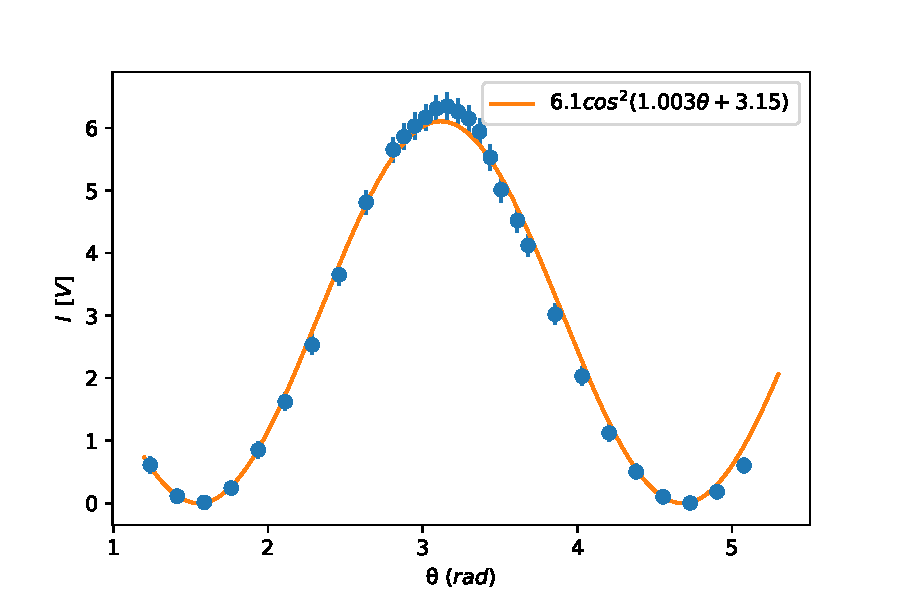
\includegraphics[width=\linewidth]{malus1.pdf}
	\captionof{figure}{\small{Voltaggio ai capi del fotodiodo in funzione dell'angolo di rotazione $\theta$ tra i due assi di polarizzazione dei filtri. Ai dati è sovrapposta la curva teorica con i parametri di fit.}}
	\label{fig:malus1}
	\end{center}
\end{Figure}

\subsection{Verifica aggiungendo un terzo polarizzatore}

Si allineano i due polarizzatori in modo da estinguere la luce proveniente dal laser, ovvero si pongono gli assi di polarizzazione ortogonali. Si interpone dunque tra essi un terzo polarizzatore, ruotato di un angolo che sarà indicato con $\theta$. Poiché non si dispone di tre polaroid, si utilizza in luogo del terzo un \emph{beam-splitter}, che facendo passare solo una delle due componenti TE o TM del fascio incidente si comporta in modo analogo ad un polarizzatore; è dunque rispetto all'asse del beamsplitter che si pone ortogonalmente l'asse del primo polaroid. Si adotta quale $\theta = 0$ l'angolo per cui si ha estinzione completa del fascio laser; si ruota dunque il polaroid interposto e si misura l'intensità della luce al variare di $\theta$. La configurazione è illustrata in Figura~\ref{fig:diagrammaMalus2}.

In questo caso l'andamento previsto è
\begin{equation}\label{eq:Malus2}
I = \frac{I_0}{4}\sin^2(2\theta),
\end{equation}
dove $I_0$ indica l'intensità della luce che raggiunge il primo filtro polarizzatore.

Si riportano in Figura~\ref{fig:malus2} i punti sperimentali ottenuti al variare dell'angolo $\theta$, a cui è sovrapposta la curva teorica data dalla~(\ref{eq:Malus2}): in questo caso, infatti, un fit necessiterebbe di una modello teorico per la variazione dell'ampiezza, che preveda infatti massimi di diversa entità, non periodici di periodo $\pi / 2$. Si ritiene che questo sia dovuto ad imperfezioni presenti sulla superficie del filtro polarizzatore, nonché alla diversa intensità delle componenti TE e TM del fascio (si veda la sezione successiva). È evidente infatti che i massimi, ad eccezione del primo e dell'ultimo, non siano riferiti alla stessa intensità. Gli altri punti sperimentali, al contrario, seguono più correttamente l'andamento teorico.

\begin{Figure}
	\begin{center}
	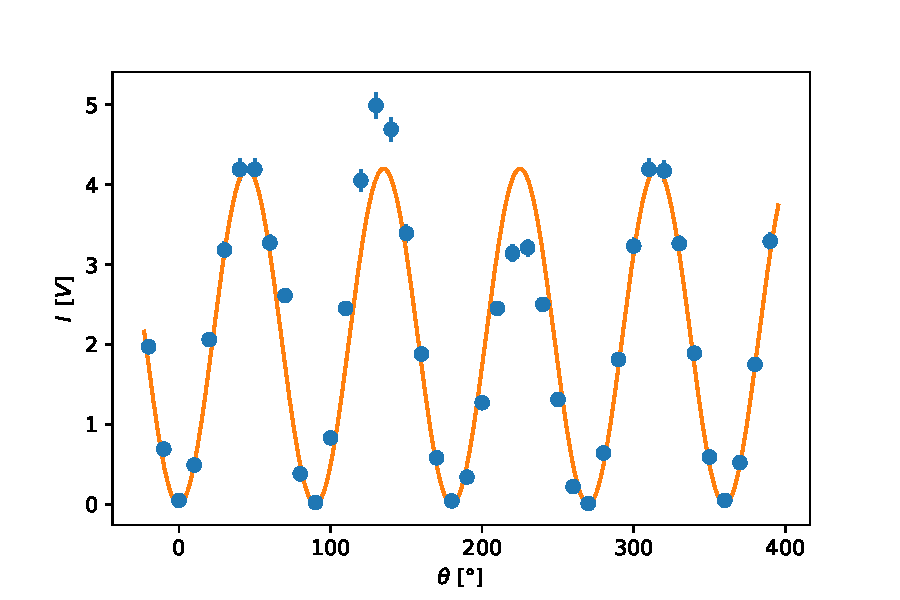
\includegraphics[width=\linewidth]{malus2.pdf}
	\captionof{figure}{\small{Voltaggio ai capi del fotodiodo in funzione dell'angolo di rotazione $\theta$ del polarizzatore interposto. Ai dati è sovrapposta la curva teorica.}}
	\label{fig:malus2}
	\end{center}
\end{Figure}

\subsection{Studio della polarizzazione del fascio in ingresso}\label{sec:polarizzazione}
Si studia l'andamento dell'intensità luminosa al variare della componente polarizzata linearmente che emerge da un singolo filtro polarizzatore. Utilizzando un singolo polarizzatore, si ruota l'asse di polarizzazione dello stesso e si misura l'intensità della luce trasmessa con il fotodiodo. In Figura~\ref{fig:single} è riportato l'andamento dell'intensità in funzione dell'angolo $\theta$ di rotazione: si osserva come essa non è costante, come dovrebbe essere nel caso di luce non polarizzata, né presenta un andamento sinusoidale, come sarebbe invece se si avesse luce polarizzata circolarmente; al contrario, i massimi di non eguale entità suggeriscono la presenza di polarizzazione ellittica, con diversa ampiezza delle due componenti ortogonali.

\begin{Figure}
	\begin{center}
	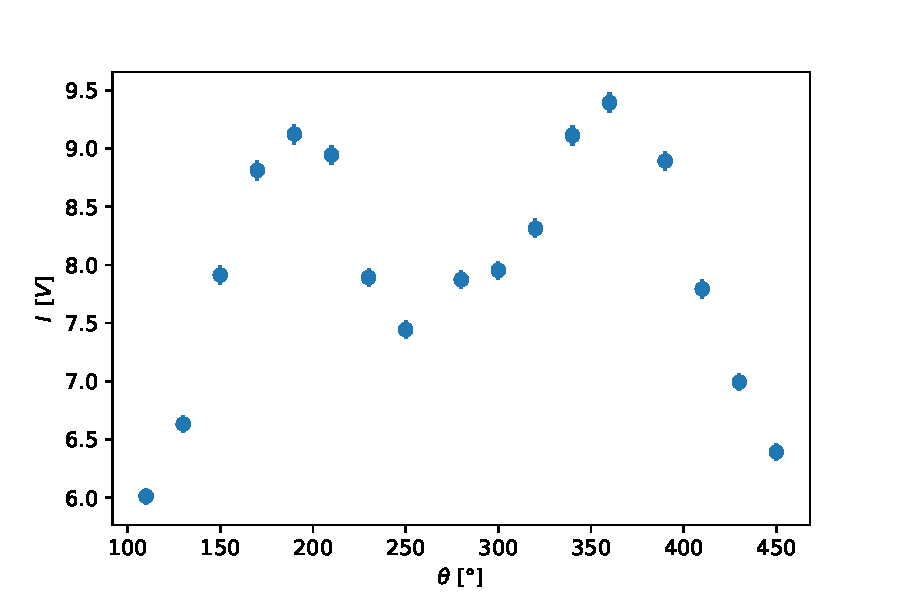
\includegraphics[width=\linewidth]{single.pdf}
	\captionof{figure}{\small{Voltaggio ai capi del fotodiodo in funzione dell'angolo di rotazione $\theta$ del singolo polarizzatore.}}
	\label{fig:single}
	\end{center}
\end{Figure}

È bene sottolineare come in questa esperienza influiscano anche il non perfetto allineamento del polaroid con il fascio incidente e la presenza di graffi o aloni sulla superficie del polaroid. Utilizzando l'espressione
\[
P = \frac{I_\text{max} - I_\text{min}}{I_\text{max} + I_\text{min}}
\]
è possibile inoltre stimare il grado di polarizzazione della luce incidente, che risulta essere compreso tra il $10$ e il $22 \%$, a seconda del massimo e del minimo scelti.





%==================================================
%             ANGOLO DI BREWSTER
%==================================================


\section{Angolo di Brewster}
Si monta l'apparato in Figura \ref{opt:brewster}, dove prima del fotodiodo è stato posizionato un \emph{beamsplitter polarizzatore}, in grado di trasmettere la componente orizzontale o quella verticale\footnote{Quale delle due componenti venga trasmessa e quale riflessa dipende da come è costruito e come è montato il beamsplitter.} della radiazione e riflettere la componente ortogonale, con coefficiente di assorbimento complessivo quasi nullo. 

Posizionando tra il beamsplitter e il rilevatore un dielettrico (perspex) in modo che il piano di incidenza del laser sia parallelo al piano di lavoro, si è verificato che la componente verticale della radiazione coincide con la componente TE e quella orizzontale con la TM: infatti per una certo configurazione del filtro polarizzatore ($\alpha_\text{TM} = \SI{52 \pm 1}{\degree}$) si ottiene che esiste un angolo di incidenza (l'\emph{angolo di Brewster}) per cui non si ha raggio riflesso. Ponendo il polaroid  all'angolo di $\alpha_\text{TE} = \alpha_\text{TM} - \SI{90}{\degree} = \SI{322 \pm 1}{\degree}$ si ottiene in uscita la sola componente TE.

Si è dunque rimosso il beamsplitter dall'apparato e si sono prese le misure di intensità del raggio riflesso dal dielettrico al variare dell'angolo di incidenza. Nel fare questo si è tenuto conto che l'intensità del laser diminuisce all'aumentare della distanza dalla sorgente a causa di fenomeni diffrattivi, quindi si è mantenuto il rilevatore sempre alla stessa distanza dal dielettrico.

Inoltre bisogna tener conto del fatto che i raggi riflessi dal dielettrico sono due: quello riflesso dalla prima superficie e quello riflesso dalla seconda. Nel fare la misura bisogna considerare che il raggio di interesse è quello corrispondente alla riflessione sulla prima superficie, riconoscibile perché associato all'angolo di riflessione minore.

Per ogni angolo di incidenza, fissato il rilevatore in modo che il fotodiodo misurasse l'intensità maggiore, si è misurata l'intensità per entrambe le componenti, ruotando il polaroid e posizionandolo sugli angoli $\alpha_{\text{TE}}$ e $\alpha_{\text{TM}}$ misurati in precedenza.

\subsection{Riflettanza}
Gli andamenti previsti per le riflettanze, ovvero i rapporti tra l'intensità misurata e quella misurata in assenza di dielettrico, sono descritti dalle due curve
\begin{equation}\label{eq:rs}
	r_{\mathrm{TE}} = r_ s = \frac{\cos \theta - \sqrt{n^2 - \sin^2 \theta}}{\cos \theta + \sqrt{n^2 - \sin^2 \theta}},
\end{equation}
\begin{equation}\label{eq:rs}
	r_{\mathrm{TE}} = r_p =  \frac{-n^2 \cos \theta + \sqrt{n^2 - \sin^2 \theta}}{n^2 \cos \theta + \sqrt{n^2 - \sin^2 \theta}},
\end{equation}
dove $n$ è il rapporto tra l'indice di rifrazione del dielettrico e quello dell'aria.
Il risultato della misura è riportato in Figura \ref{fig:brewster_I}, dove ai dati sperimentali sono sovrapposte le curve teoriche corrispondenti a $n_s = \SI{1.49 \pm 0.01}{}$ e $n_p = \SI{1.50 \pm 0.02}{}$, valori ottenuti fittando le curve sui dati sperimentali.
\begin{Figure}
	\begin{center}
	\includegraphics[width=\linewidth]{riflettanze.pdf}
	\captionof{figure}{Riflettanza delle componenti TE e TM al variare dell'angolo di incidenza, si riportano le curve teoriche fittate.}
	\label{fig:brewster_I}
	\end{center}
\end{Figure}

\subsection{Visibilità}
Per stimare l'angolo di Brewster del dielettrico, ossia l'angolo per cui l'intensità della componente TM del fascio riflesso si annulla, si studia la visibilità del fascio definita come
\begin{equation}\label{eq:visibilità}
	V(\theta) = \frac{r_s(\theta) - r_p(\theta)}{r_s(\theta) + r_p(\theta)}
\end{equation}
dalla cui definizione è evidente che
\begin{equation}
	\left. V(\theta) \right\vert_{\theta = \theta_\mathrm{Brewster}} = 1.
\end{equation}
In Figura \ref{fig:brewster_V} sono riportati i dati sperimentali insieme alla curva teorica corrispondente a $n_V = \SI{1.61 \pm 0.04}{}$, ottenuto fittando i dati.
\begin{Figure}
	\begin{center}
	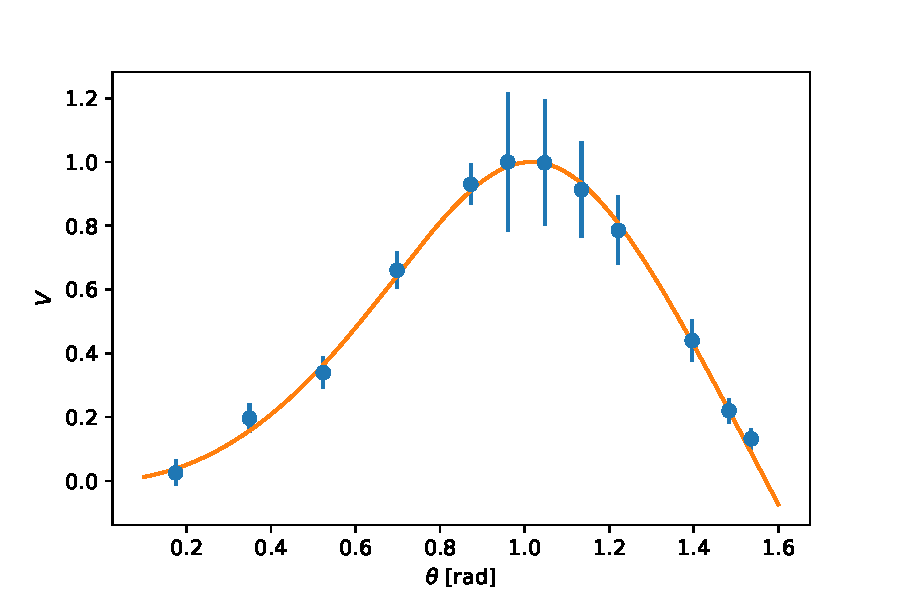
\includegraphics[width=\linewidth]{visibilità.pdf}
	\captionof{figure}{Visibilità del raggio riflesso, si riporta la curva teorica fittata.}
	\label{fig:brewster_V}
	\end{center}
\end{Figure}
Si nota che i diversi valori di $n$ ottenuti in quest'ultima parte dell'esperienza sono incompatibili tra loro, ciò è sintomo di una sottostima delle incertezze sui valori di intensità.
Per stimare l'angolo $\theta_\mathrm{max}$ corrispondente al massimo della visibilità, si fa una media trai due angoli corrispondenti ai valori misurati della visibilità più alti, si ottiene
\begin{equation}
	\theta_\mathrm{max} = \theta_\mathrm{brewster} = \SI{57 \pm 2}{°}
\end{equation}
da cui, essendo 
\begin{equation}
	\theta_\mathrm{brewster} = \arctan (n)
\end{equation}
si trova 
\begin{equation}
	n = \tan (\theta_\mathrm{brewster} )= \SI{1.54 \pm 0.05}{},
\end{equation}
compatibile con i valori ottenuti precedentemente.

\end{multicols}




%ESEMPIO DI FIGURA
%\begin{Figure}
%	\begin{center}
%	\includegraphics[width=\linewidth]{comune.png}
%	\captionof{figure}{Istantanea dell'oscilloscopio per l'amplificatore differenziale, misura di $A_c$}
%	\label{fig:Ac_differenziale}
%	\end{center}
%\end{Figure}


%ESEMPIO DI TABELLA
%\begin{center}
%\captionof{table}{Misure per la stima di $A_c$}
%\label{tab:Ac_differenziale}
%\begin{tabular}{c|c|c|c}
%$f$ [\SI{}{Hz}] & $V_i$ [\SI{}{V}] & $v_o$ [\SI{}{mV}] & $A_c = v_o / V_i$ \\
%\hline
%      149.5 &        3.90 &         11.3 & 2.90e-03 \\
%      222.0 &        3.90 &         11.5 & 2.95e-03 \\
%      281.0 &        3.90 &         11.8 & 3.03e-03 \\
%      359.0 &        3.90 &         11.8 & 3.03e-03 \\
%      461.0 &        3.90 &         12.2 & 3.13e-03 \\
%\hline
%\end{tabular}
%\end{center}


\end{document}
